\section{Тренировочное задание}

Заполняем ресурсный лист исполнителями и материальным ресурсом.

\begin{figure}[H]
	\centering
	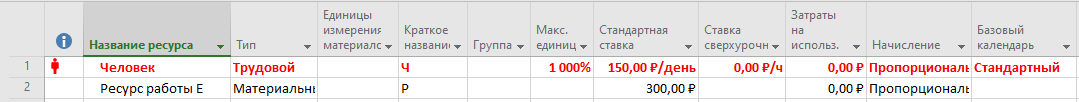
\includegraphics[width=0.8\textwidth]{img/content/resources_0.png}
	\caption{Ресурсы тренирововчного задания}
\end{figure}

Далее назначаем ресурсы на задачи.

\begin{figure}[H]
	\centering
	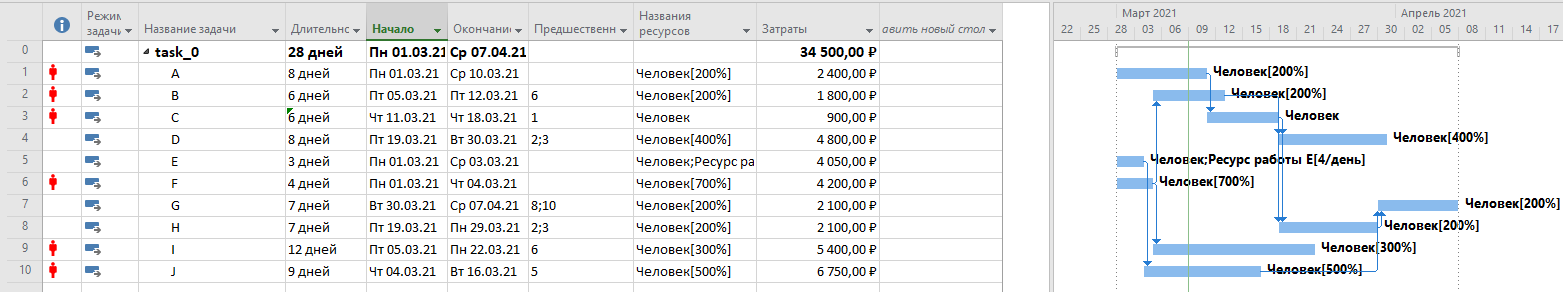
\includegraphics[width=0.8\textwidth]{img/content/resources_tasks_0.png}
	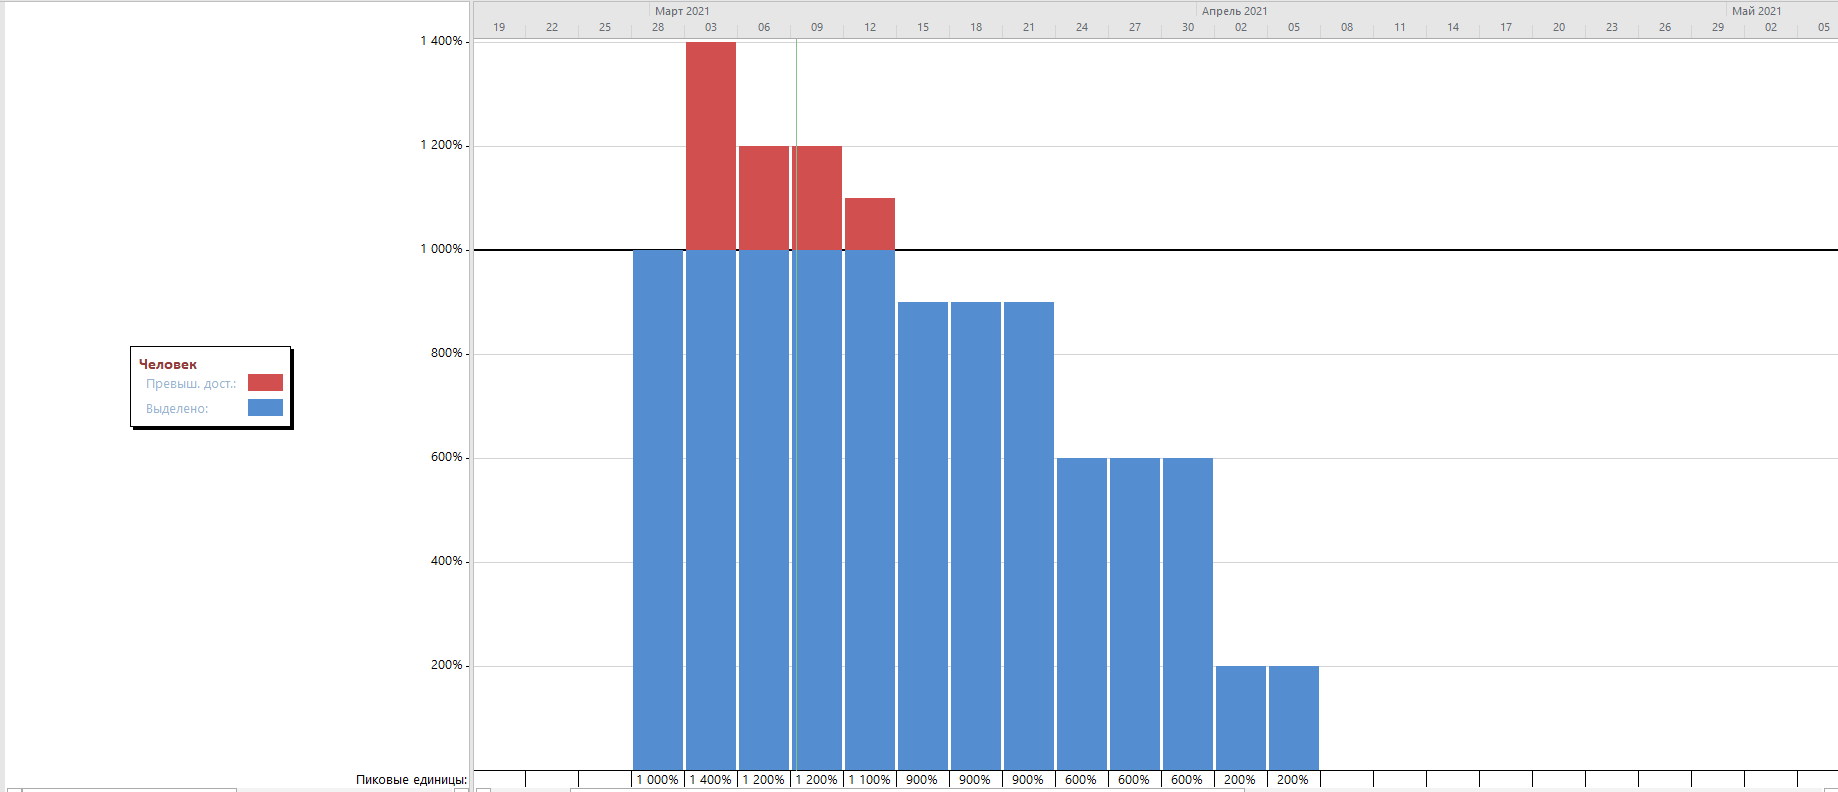
\includegraphics[width=0.8\textwidth]{img/content/graph_recourses_0.png}
	\caption{Распределение ресурсов по задачам}
\end{figure}

Ресурсы перегружены на 400 \%.

\section{Условие задания}

Содержание проекта: Команда разработчиков из 16 человек занимается созданием карты города на основе собственного модуля отображения. Проект должен быть завершен в течение 6 месяцев. Бюджет проекта: 50 000 рублей.

\section{Задание 1}

Заполняем ресурсный лист.

\begin{figure}[H]
	\centering
	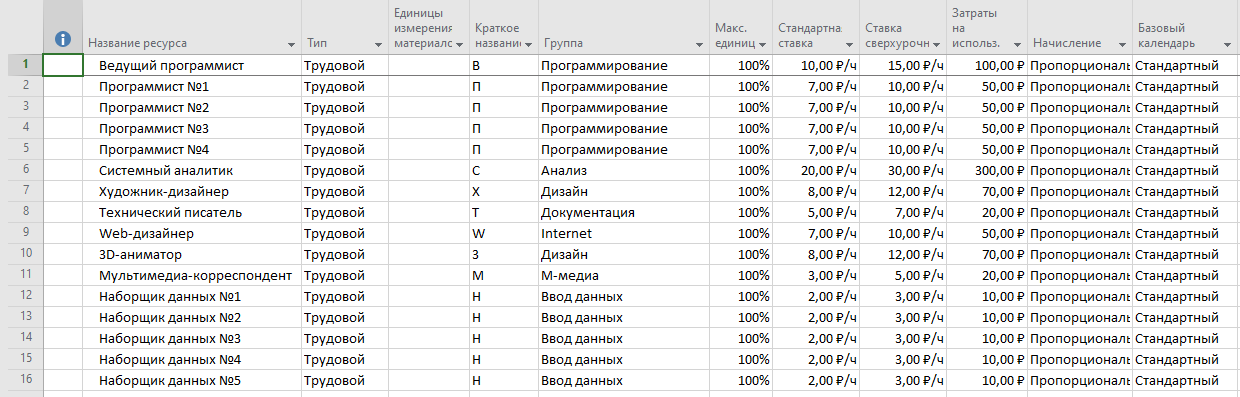
\includegraphics[width=0.8\textwidth]{img/content/resources.png}
	\caption{Лист ресурсов}
\end{figure}

\section{Задание 2}

Назначаем ресурсам задачи. Дополнительно для задачи 8 арендуем сервер (он работает 24 часа в сутки).

\begin{figure}[H]
	\centering
	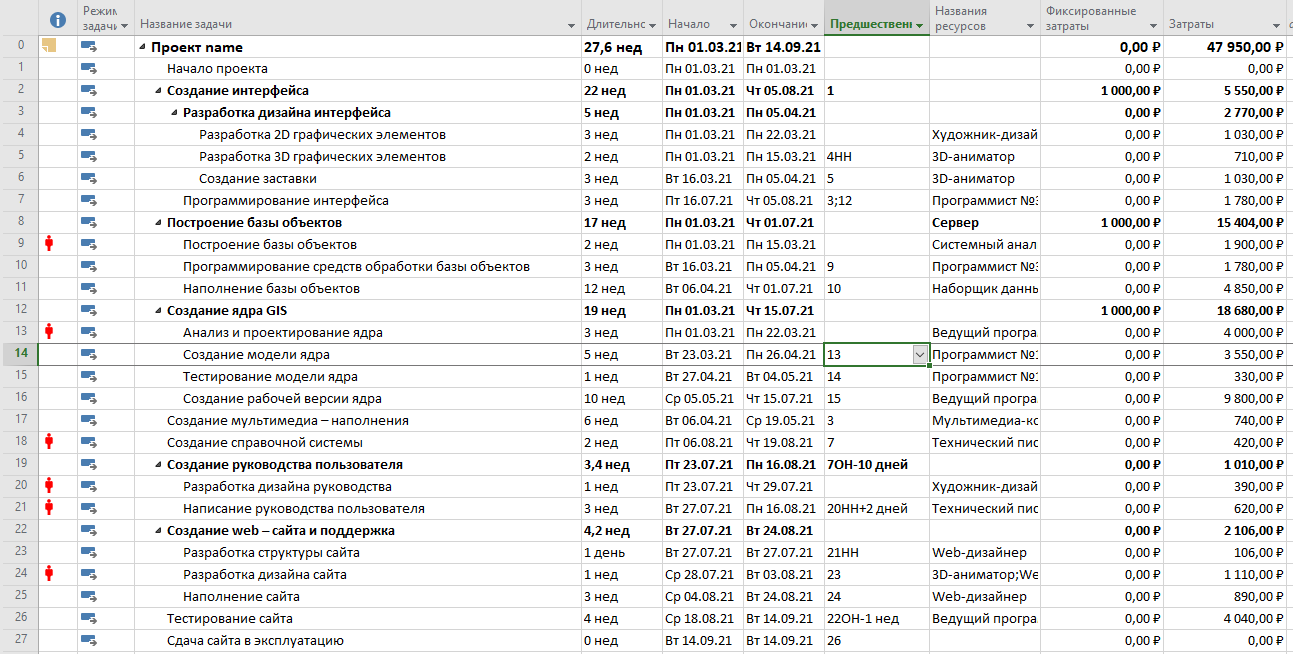
\includegraphics[width=0.8\textwidth]{img/content/resources_tasks.png}
	\caption{Распределение ресурсов по задачам}
\end{figure}

Перегрузка ресурсов:

\begin{itemize}
	\item Системный аналитик – одновременно выполняет задачи 9 (Анализ и построение структуры базы объектов ) и 13 (Анализ и проектирование ядра).
	\item Технический писатель – одновременно выполняет задачи 21 (Написание руководства пользователя) и 18 (Создание справочной системы).
	\item Художник-дизайнер – одновременно выполняет задачи 20 (Разработка дизайна руководства) и 24 (Разработка дизайна сайта).
\end{itemize}

\begin{figure}[H]
	\centering
	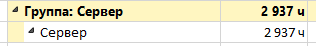
\includegraphics[width=0.8\textwidth]{img/content/server.png}
	\caption{Использование ресурса сервер}
\end{figure}

Добавим фиксированные затраты для задач 2, 8 и 12.

\begin{figure}[H]
	\centering
	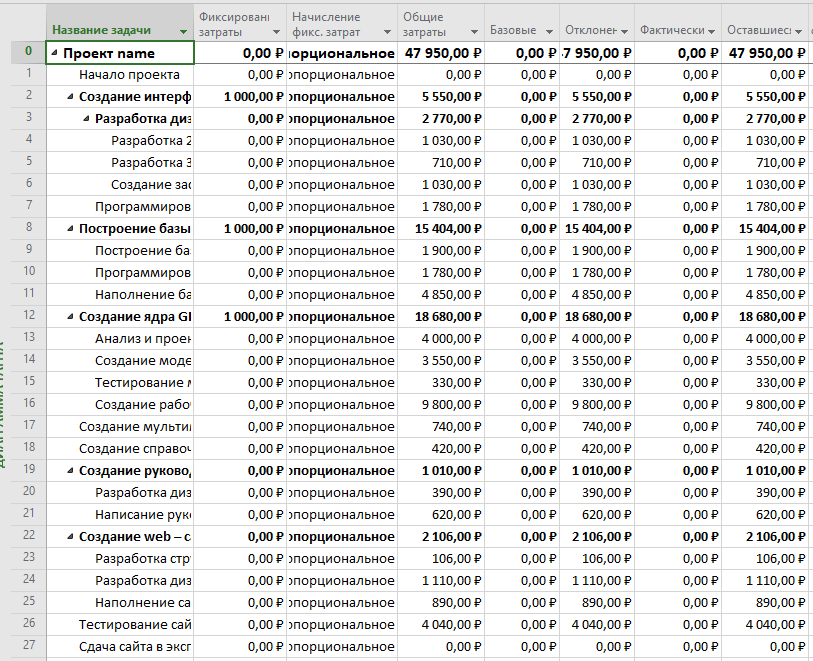
\includegraphics[width=0.8\textwidth]{img/content/money.png}
	\caption{Затраты задач}
\end{figure}

\section{Задание 3}

Анализ затрат по группам ресурсов.

Заходим в представление Использование ресурсов и устанавливаем группировку.

\begin{figure}[H]
	\centering
	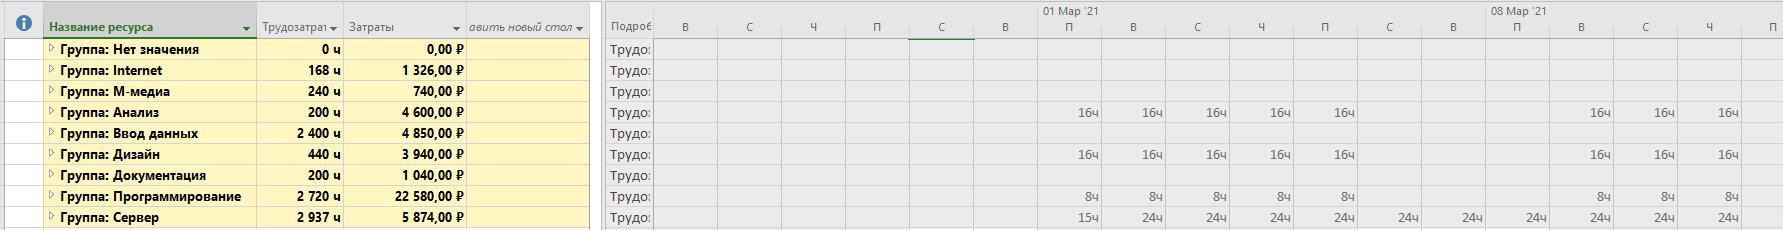
\includegraphics[width=0.8\textwidth]{img/content/groups.png}
	\caption{Затраты по группам ресурсов}
\end{figure}

Для графического представления воспользуемся MS Excel.

\begin{figure}[H]
	\centering
	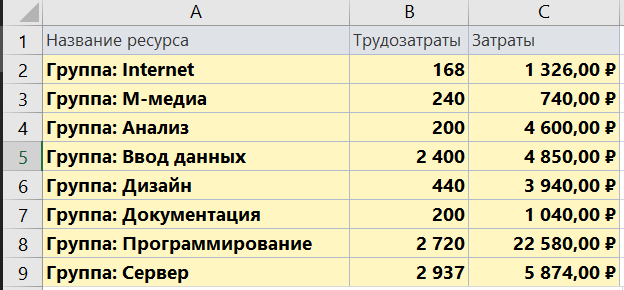
\includegraphics[width=0.8\textwidth]{img/content/table.png}
	\caption{Затраты по группам ресурсов}
\end{figure}

\begin{figure}[H]
	\centering
	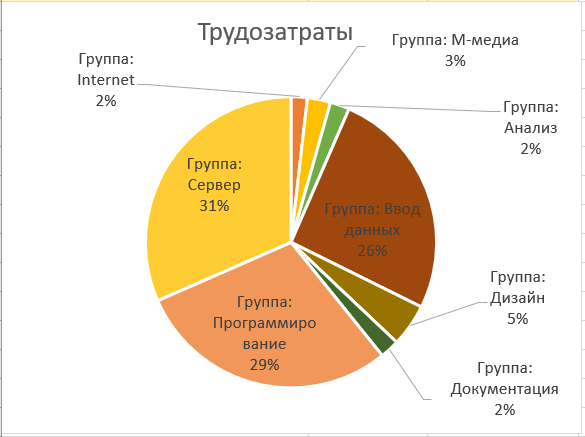
\includegraphics[width=0.8\textwidth]{img/content/diagram_hours.png}
	\caption{Информация о трудозатратах по структурным группам ресурсов}
\end{figure}

\begin{figure}[H]
	\centering
	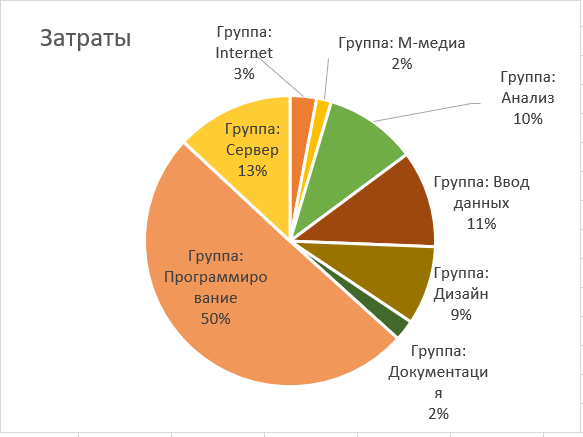
\includegraphics[width=0.8\textwidth]{img/content/diagram_money.png}
	\caption{Информация о затратах по структурным группам ресурсов}
\end{figure}

Как видим, на программистов приходится большая часть и затрат 50\%, и трудозатрат 29\%.

На сервер приходится 13\% затрат.

Также одной из больших затрат является аналитик 10\%, хотя выполняет
всего 2\%.

Также затраты на ввод данных (наборщиков текста) составляют 11\% от общего бюджета, несмотря на то, что они выполняют 26\% работы.

Во всех остальных случаях объем работ и деньги в процентном соотношении примерно эквивалентны.


\section{Вывод}

В ходе выполнения лабораторной работы №2 продолжается изучение основных возможностей Microsoft Project 2019. Были созданы списки ресурсов, назначены ресурсы задачам и проведен анализ затрат по группам ресурсов.

В результате было выяснено, что программный проект укладывается в выделенный бюджет (47 950 рублей из 50 000 рублей). Но остается совсем небольшой запас денег, также системный аналитик, художник-дизайнер и технический писатель перегружены.
